\chapter{\leavevmode \newline Introduction}
\label{chap:Introduction}

The future of space exploration increasingly relies on our ability to establish a sustainable human presence beyond Earth. As missions become more ambitious, with visions of long-term habitation on the Moon, Mars, and other celestial bodies, the importance of robust robotic systems capable of autonomous exploration becomes ever more critical. Before building the infrastructure that future astronauts will depend on, we must first navigate and understand unfamiliar and often hazardous terrains, frequently without direct human supervision.

For decades, wheeled rovers have served as humanity’s primary tools for planetary exploration. Their successes, such as Spirit and Opportunity’s extensive traverses across the Martian surface and Curiosity and Perseverance's ongoing missions, have significantly expanded our knowledge of other worlds. However, as we move toward the goal of sustained human presence, the limitations of traditional rovers have become increasingly apparent. These systems depend heavily on human oversight and primarily on camera-based sensors, interpreting their environment largely through visual data. While vision provides rich spatial information, it offers only an indirect understanding of the terrain.

This reliance on vision presents significant risks when operating in granular, deformable environments. Materials such as regolith, volcanic ash, and fine particulate dust, which are common on planetary surfaces, can be deceptive. Two patches of ground may appear identical but respond very differently under load. One may be stable and supportive, while the other collapses under minimal pressure. Cameras, regardless of resolution or sophistication, are inherently limited in their ability to infer critical mechanical properties such as cohesion, bearing strength, or subsurface instability.

A poignant reminder of these challenges comes from the story of the Spirit rover, which in 2009 became irretrievably stuck in Martian sand despite careful navigation. The episode captured public attention and was memorialized in popular culture, such as in XKCD’s comic tribute \cite{xkcdspirit}:

\begin{figure}[htbp]
    \centering
    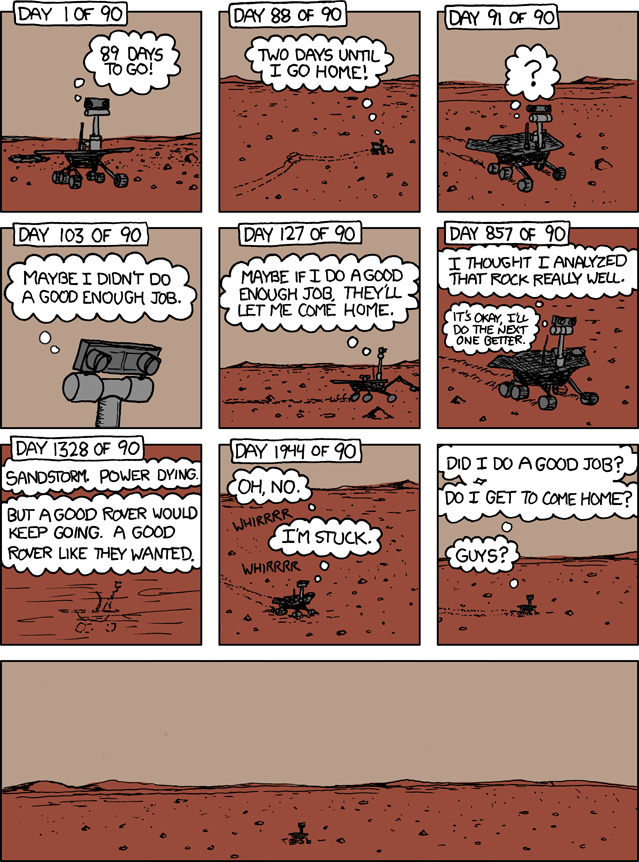
\includegraphics[width=0.7\linewidth]{figures/xkcd_spirit.png}
    \caption{XKCD comic \#695: A tribute to Spirit, highlighting the emotional weight and technical challenge of navigating granular terrain \cite{xkcdspirit}.}
    \label{fig:xkcd_spirit}
\end{figure}

Though humorous in style, the comic conveys a sense of quiet tragedy. It conveys the undeniable truth: our robotic explorers are vulnerable to many hazards when faced with environments they cannot fully perceive or understand.

Moreover, granular terrains are dynamic and can change significantly across distances. Small disturbances, such as the pressure from a robot’s wheel or foot, can cause localized deformation, slippage, or collapse. These changes often occur without any visual indication. Dust accumulation and variable lighting conditions, including low sun angles and deep shadows, further complicate visual perception, making reliance on vision alone increasingly dangerous.

Recognizing these challenges, a new paradigm for planetary exploration is necessary, one that moves beyond passive observation to active physical interrogation of the environment. NASA’s Legged Autonomous Surface Science In Analogue Environments (LASSIE) project \cite{Fisher2023LASSIE} embodies this approach. Instead of simply observing, legged robots interact with the terrain, using their limbs not only for locomotion but also as scientific instruments capable of performing mechanical tests.

Legged robots offer a unique advantage for such interactions. Every step becomes an opportunity to measure the mechanical response of the terrain. By pressing into the surface, applying controlled forces, and recording the resulting displacements, these robots can infer properties such as stiffness, cohesion, and internal friction. Unlike visual sensing, which depends on interpreting surface features, proprioceptive sensing provides direct measurements of terrain characteristics critical to safe navigation and environmental understanding.

\begin{figure}
    \centering
    \includegraphics[width=0.5\linewidth]{figures/202308_LASSIE_MT_HOOD_DAY4_A_3880.jpg}
    \caption{Ghost Robotics Spirit, the quadrupedal robot used in LASSIE experiments on Mount Hood.}
    \label{fig:spiritrobot}
\end{figure}

The LASSIE project’s quadrupedal platforms, such as the Ghost Robotics Spirit shown in \autoref{fig:spiritrobot}, are equipped with actuators capable of precise force control. These robots systematically perform mechanical measurements during locomotion, continuously gathering data about the terrain they traverse.

\begin{figure}
    \centering
    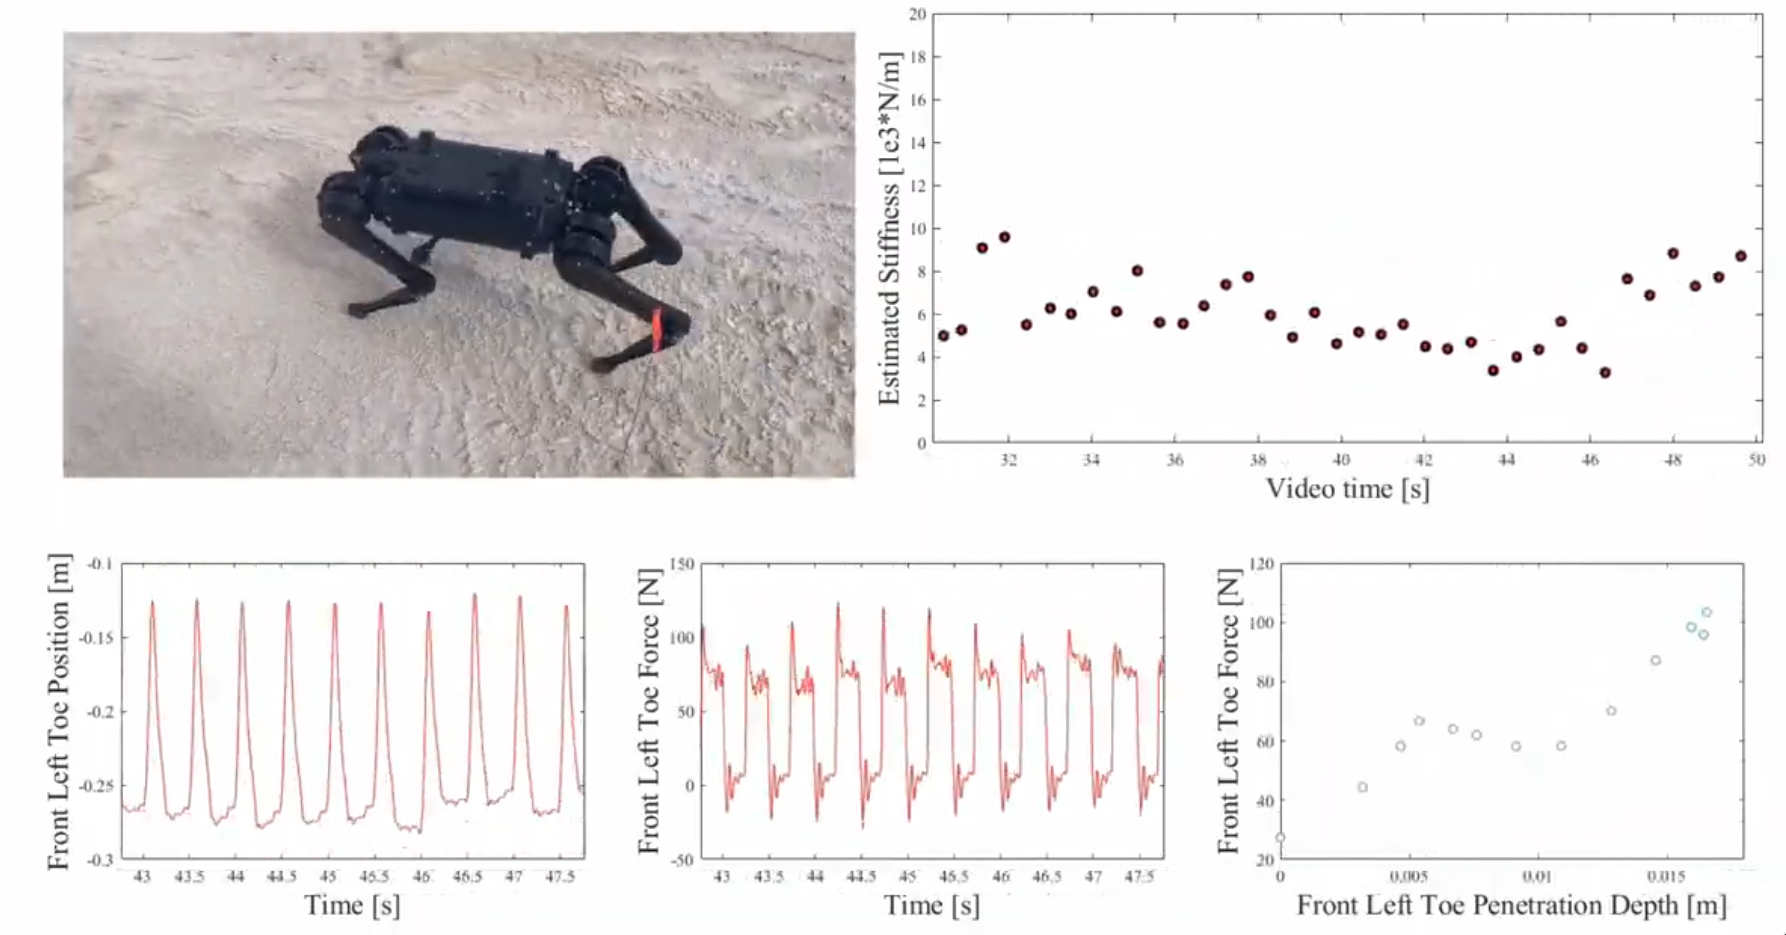
\includegraphics[width=0.8\linewidth]{figures/proprioceptive_sensing.png}
    \caption{A LASSIE quadrupedal robot recording terrain stiffness during each step.}
    \label{fig:proprioceptive-sensing}
\end{figure}

As shown in \autoref{fig:proprioceptive-sensing}, each step provides new information about terrain stiffness and stability. These measurements not only ensure the safety of the robot’s immediate movements but also build a continuously updated map of the environment. Over time, the robot constructs a detailed understanding of the traversability and mechanical behavior of the landscape.

Several challenges remain in leveraging proprioceptive sensing for autonomous navigation. Most existing navigation algorithms are designed with the assumption that the robot has access to either global terrain maps or rich local sensing from sources such as LIDAR or cameras. These sensors provide spatial context beyond the robot’s current location, allowing planners to construct paths based on look-ahead information. In contrast, proprioceptive sensing is inherently localized. The robot receives information only at the exact point of contact with the terrain, with no visibility into the safety of neighboring or distant regions.

This limitation introduces several technical challenges:

\begin{enumerate}
    \item \textbf{Sparse and Delayed Observability:} Because the robot can only sense terrain after physically interacting with it, the environment must be discovered incrementally and cautiously.
    \item \textbf{Uncertainty in Terrain Modeling:} Local measurements are subject to noise and variability, making it difficult to construct a reliable global map of terrain safety.
    \item \textbf{Balancing Exploration and Exploitation:} The robot must decide whether to explore unknown regions to reduce uncertainty or exploit known safe areas to reach the goal, while maintaining a margin of safety.
    \item \textbf{Real-Time Decision Making:} Planning must occur under strict time constraints and be continuously updated in response to new measurements.
    \item \textbf{Safety Guarantees with Minimal Lookahead:} Without visibility into terrain ahead, the robot must ensure safety using only current and past measurements.
\end{enumerate}

This thesis builds upon the LASSIE exploration loop by introducing a navigation strategy called \textit{\algonamefull{}} (\algoname{}) that places proprioceptive sensing at the core of the robot’s decision-making process. \algoname{} enables the robot to use each proprioceptive measurement to inform both its immediate path planning and its broader exploration objectives. Specifically, \algoname{} generates safe, dynamically updated paths based on local terrain measurements, while also selecting optimal locations for conducting further mechanical tests. Through this active exploration loop, the robot incrementally expands its map of traversable terrain while minimizing risk.

Through the integration of proprioceptive measurements and adaptive navigation, this research aims to transform the process of planetary exploration from a passive visual survey to an active, resilient, and intelligent engagement with the environment. Such capabilities are not technological conveniences but essential requirements for building a sustainable human presence beyond Earth.

The remainder of this thesis is organized as follows. Chapter~\ref{chap:Literature Review} provides a literature review of related work in autonomous navigation. Chapter~\ref{chap:Methods} details the proposed methodology, including the design of the \algoname{} framework and its integration into the LASSIE exploration loop. Chapter~\ref{chap:Results} presents the simulation setup and interprets simulation results. Finally, Chapter~\ref{chap:Discussion} analyzes limitations of \algoname{}, and outlines opportunities for future research.
